%%%%%%%%%%%%%%%
% CH2 %
%%%%%%%%%%%%%%

\chapter{The 2D airfoil}
	\section{Nomenclature}
		
		\begin{center}
		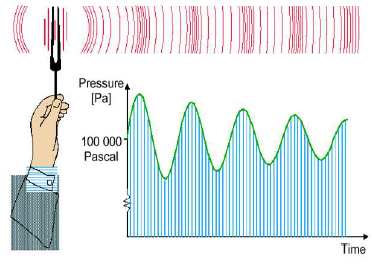
\includegraphics[scale=1]{ch2/1}
		\captionof{figure}{}
		\end{center}
		
		The connection between the trailing edge and the leading edge is called the \textbf{chord}. Then we have a \textbf{camber line} which is the line following the shape of the foil. The thickness is always normal to the camber line. Let's note that the camber line and the thickness distribution are function of the position $f(x)$. \\
		
		Eastman Jacobs created around 1930 a family of wing profiles, known as the NACA profiles. He characterised them by 4 digit numbers: 
		
		\begin{itemize}
			\item[•] The first is the \textbf{maximum camber in percentage of the chord} 
			\item[•] The second is the \textbf{position of the maximum camber in 1/10 percentage of the chord}
			\item[•] The last two digits gives the \textbf{position of the maximum thickness in percentage of the chord}\\
		\end{itemize}				
		
		These were characterizing the 2D representation, but a wing is 3D. We have also the \textbf{wing surface S}, \textbf{the span of the wing b} and we can define a mean chord as: 
		\begin{equation}
		<c> = \frac{S}{b}.
		\end{equation}				
		 For civil aircraft, b/c is between 6-10 and for glider b/c = 12, this is called the \textbf{aspect ratio} (slenderness ratio). 
		 
		 \newpage
		 
	\section{The flow around 2D airfoils}
		
		\begin{wrapfigure}[9]{l}{7.5cm}
		\vspace{-5mm}
		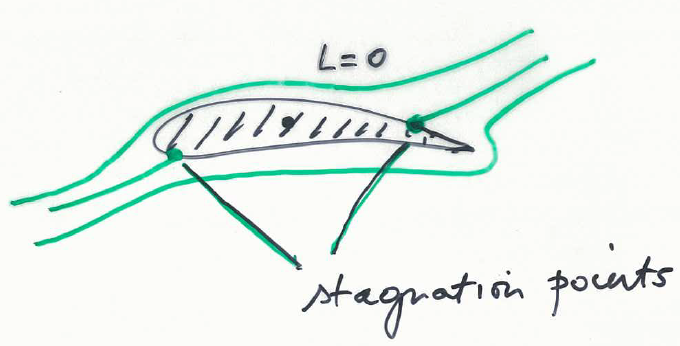
\includegraphics[scale=0.35]{ch2/3}
		\captionof{figure}{}
		\label{fig:2.2}
		\end{wrapfigure}
		Let's remind the expression of the force applied on the wing:
		
		\begin{equation}
		\vec{R} = -\oint p \, d\vec{S} + \oint \bar{\bar{\tau}} \, d\vec{S} 
		\end{equation}
		
		with an external normal to the airfoil. The angle of attack is represented on \autoref{fig:2.2}.

		The pressure term is responsible for lift and the friction term is responsible for drag. Friction forces work tangential to the airfoil and the pressure forces are perpendicular, if there is \textbf{no separation} in the flow. 
		Note that in a subsonic inviscid incompressible flow, we have the paradox of d’Alembert because we have no drag. This shows that the pressure only contributes to lift. \\

		What happens when we have \textbf{separation} is that we have a region above the airfoil where $p-p_\infty \approx 0$ and so we have a very big pressure below $p\gg p_\infty$ that slows down the wing. This implies that the applied force is higher than the case without separation and due to the attack angle, the drag force too. This phenomenon is called \textbf{pressure drag} (form drag), and here the pressure contributes to drag.
		
		\begin{center}
		ADD FIGURE 4
		\end{center}
		
		\begin{wrapfigure}[15]{r}{6cm}
		\vspace{-5mm}
		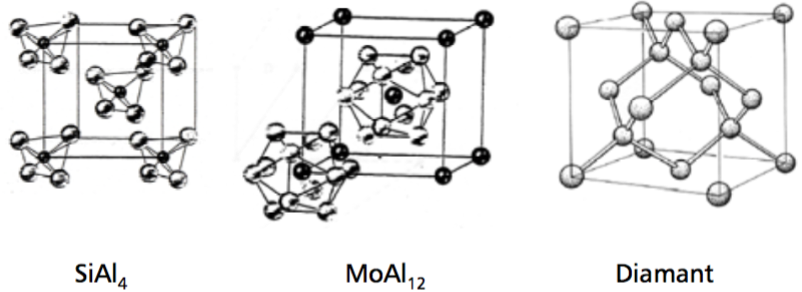
\includegraphics[scale=0.4]{ch2/2}
		\captionof{figure}{}
		\end{wrapfigure}
		The figure shows how the geometry of the body influence the drag force which can be sometimes principally caused by pressure. If we have a flat plate or a cylinder we have a huge separation, so principally a form drag $D_f$. We will have less pressure drop with the wing profile as it perfectly follows the flow direction, to end up smoothly, in this case the friction drag $D_f$ is more important. This shows the importance of profiles. \\
		
		If we look to the weight of a plane, it is surprising to see the importance of lift force. This is possible thanks to the high \textbf{atmospheric pressure}. Indeed, the wing load is defined as: 
		
		\begin{equation}
		\mbox{wing load} = \frac{\mbox{weight plane}}{\mbox{surface aera wings}}
		\end{equation}
				
		and this is commonly approximately equal to 5000 Pa = 500 $kg/m^2$. This can be easely reached by a small perturbation of the atmospheric pressure ($10^5$Pa $\rightarrow$ $5\% = 5000$ Pa). \\
		
		\subsection{Distribution of the pressure coefficient}
			Let's see the effect of the angle of attack. For small angles, we can neglect the force derivation implied and consider it to be perpendicular to the chord. This allows to neglect the drag component (refer to \autoref{fig:2.2}). If we assume that $v$ is in the x direction, the lift force approximation is:
			
			\begin{equation}
			R_y = - \oint p \, d\vec{S}.\vec{1}_y = - \oint p \, dS_y.
			\end{equation}						
			 
			The lift force is fully created by pressure and we can call the lower part of the wing the \textbf{pressure side} and the upper part the \textbf{suction side}. 
			
			\begin{wrapfigure}[11]{l}{8cm}
			\vspace{-5mm}
			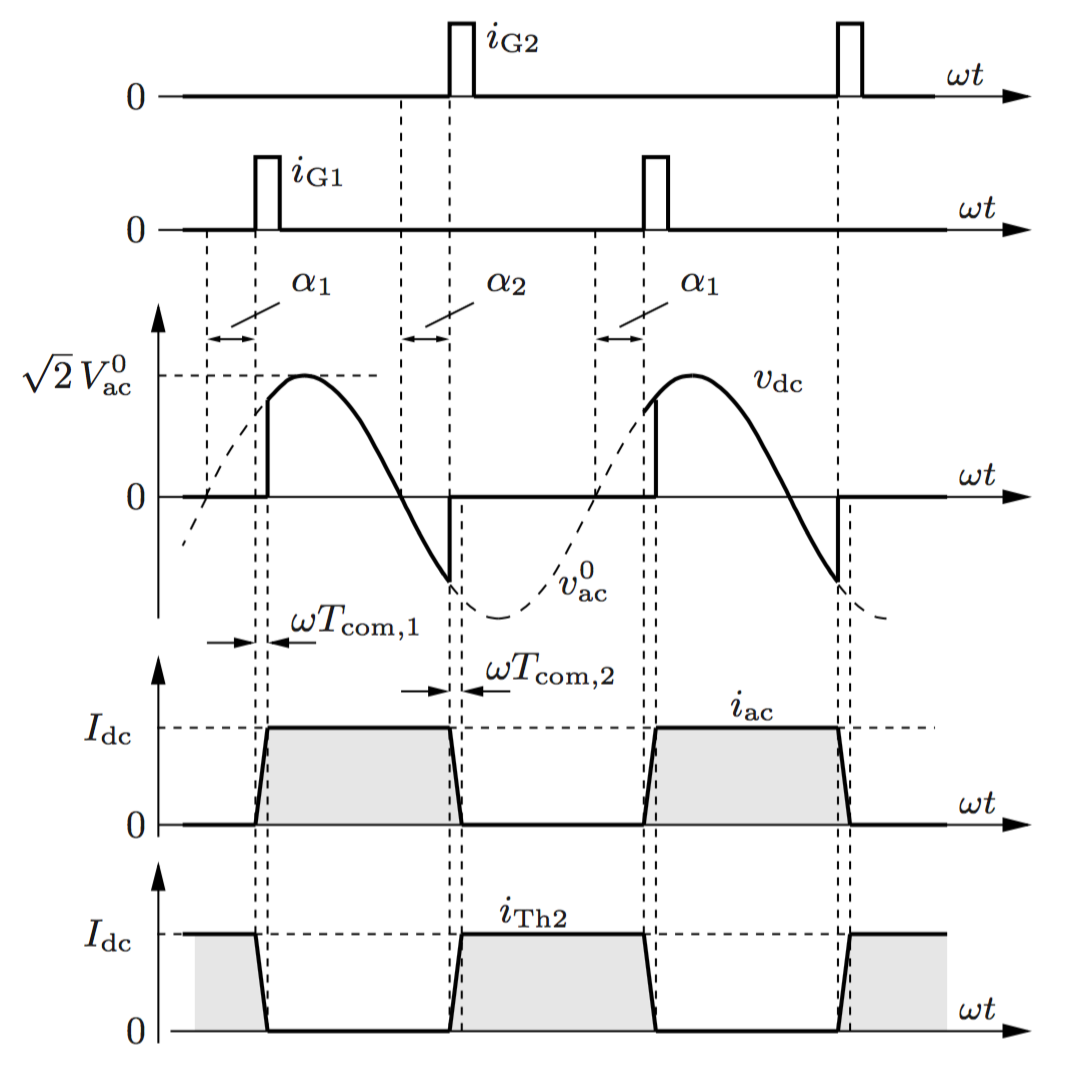
\includegraphics[scale=0.4]{ch2/4}
			\captionof{figure}{}
			\label{fig:2.4}
			\end{wrapfigure}
			The suction effect is always bigger than the pressure one. We introduce the pressure coefficient $C_p = \frac{p-p_\infty}{\frac{1}{2}\rho v_\infty ^2}$ which direction points always down! The pressure side is the green curve below and the suction side is the green curve on the upper side of \autoref{fig:2.4}. \\

			If we look to the leading edge, we have a tendency to go to $C_p = 1$. Indeed, if we write Bernouilli along a streamline and take into account the stagnation point where $v=0$, we have:
			
			\begin{equation}
			p_\infty + \rho \frac{v_\infty ^2}{2} = cst = p_{LE} + 0 \qquad \Rightarrow C_p = \frac{p_{LE}-p_\infty}{\frac{1}{2}\rho v_\infty ^2} = 1.
			\end{equation}						
			
			The pressure recovery means that we will have again $p = p_\infty$ at that point. At the leading edge this is the case because it is commonly a stagnation point. \\ 

For the trailing edge we have two cases. If it is \textbf{blunt} trailing edge, we have the $C_p = 1$ case (leading edge always blunt). If we have a \textbf{sharp} trailing edge, we will have $v_\infty$ at the previous stagnation point and so the Bernouilli equation rewrites:

			\begin{equation}
			p_\infty + \cancel{\rho \frac{v_\infty ^2}{2}} = cst = p_{TE} + \cancel{\rho \frac{v_\infty ^2}{2}} \qquad \Rightarrow C_p = \frac{p_{TE}-p_\infty}{\frac{1}{2}\rho v_\infty ^2} = 0.
			\end{equation}
			
			\begin{wrapfigure}[7]{r}{8cm}
			\vspace{-5mm}
			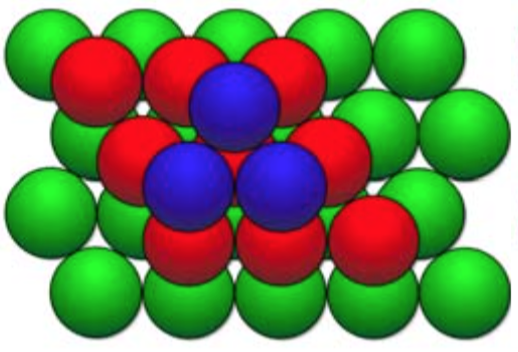
\includegraphics[scale=0.5]{ch2/5}
			\captionof{figure}{}
			\end{wrapfigure}
			We have a very big expansion on the LE (separation), so this induces a suction peak as the pressure falls above and increases below. Then we go back to the normal pressure. Let’s remind that decreasing pressure is favourable because the flow stays attached but if we have pressure increase, it's unfavourable, because we risk separation.
The angle of attack is important because the flow has more difficulties to turn on the LE  when angle goes up so the separation and the sucking peak are more important.\\

			This case is particular because the rear is reversed, so the pressure side becomes sucking and inversely. The reduced camber and reduced thickness makes the wing more vulnerable to angle change.
			
			\begin{wrapfigure}[2]{l}{7.5cm}
			\vspace{-5mm}
			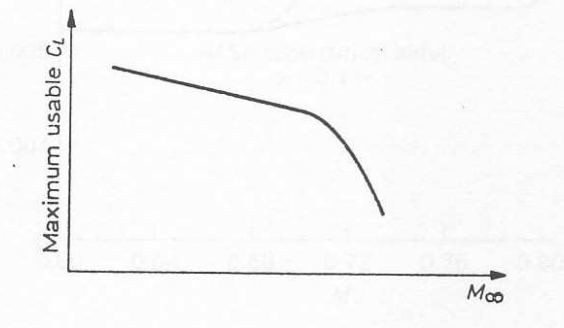
\includegraphics[scale=0.5]{ch2/6}
			\captionof{figure}{}
			\end{wrapfigure}
			Natural laminar section. The smoother LE reduces the peak and the sharp TE induces $C_p = 0$.\\\\
			
			\begin{wrapfigure}[2]{r}{7.5cm}
			\vspace{-5mm}
			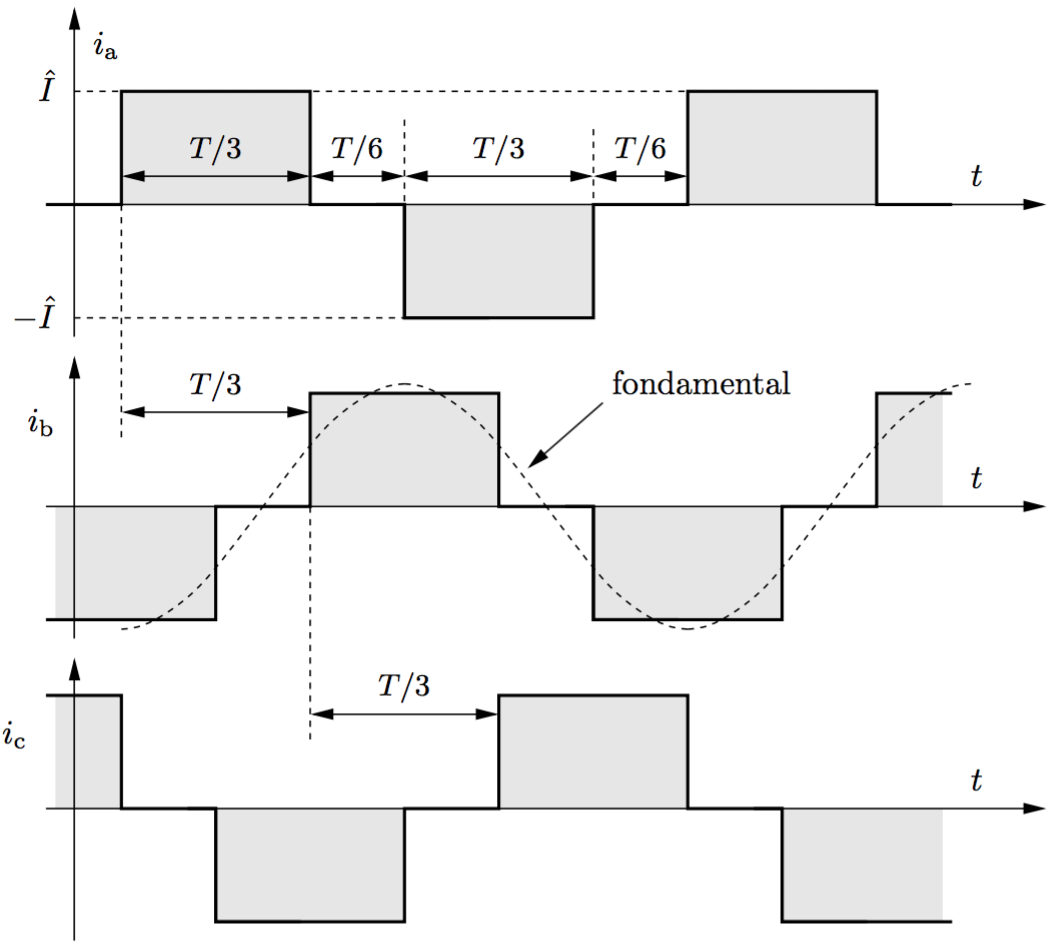
\includegraphics[scale=0.5]{ch2/8}
			\captionof{figure}{}
			\end{wrapfigure}
			This is a symetrical shape and thus only one line is shown. The thickness makes it more resistible to angle change. \\\\\\
			
			\begin{wrapfigure}[2]{l}{7.5cm}
			\vspace{-5mm}
			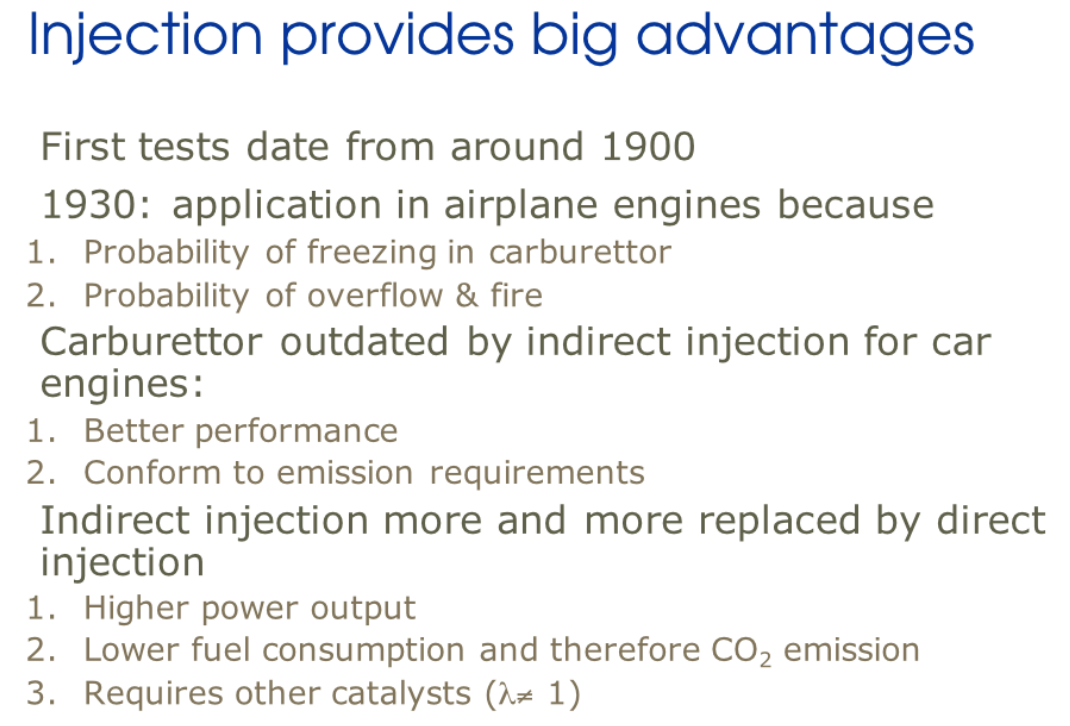
\includegraphics[scale=0.5]{ch2/9}
			\captionof{figure}{}
			\end{wrapfigure}
			Even if the wing is thin, the camber makes it more suited to high attack angle. \\\\\\
		
		\section{Center of pressure, moment and aerodynamic center}
			\subsection{Center of pressure and moment}
				\subsubsection{Calculation of lift force}
					\begin{wrapfigure}[12]{r}{3.5cm}
					\vspace{-5mm}
					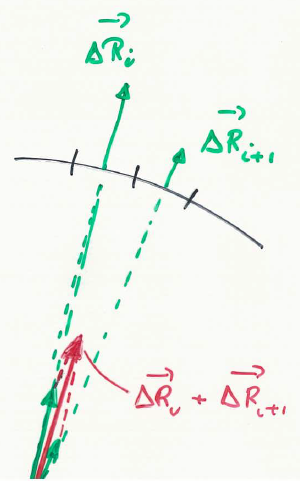
\includegraphics[scale=0.4]{ch2/10}
					\captionof{figure}{}
					\end{wrapfigure}
					We can calculate the lift by $L = \rho v_\infty \Gamma$, but we need the $\Gamma$ which is not calculable. So we will use the trick that consist in forgetting the drag term in the $\vec{R}$. Then we integrate the pressure around the surface:
					
					\begin{equation}
					\vec{R} = -\oint p \, d\vec{S} = - \sum \underbrace{p_i \vec{\Delta S_i}}_{\Delta R_i}
					\end{equation}
					
				\subsubsection{Center of pressure}
					It's the x value on the chord where the carrier of the force $\vec{R}$ intersects the chord. It's function of the angle of attack. Indeed, if alpha increases, the suction peak will be higher, this induces that the center of pressure move forward (participation of the forward pressure more important).
					
				\subsubsection{Equivalent forces}
					\begin{wrapfigure}[7]{l}{3cm}
					\vspace{-5mm}
					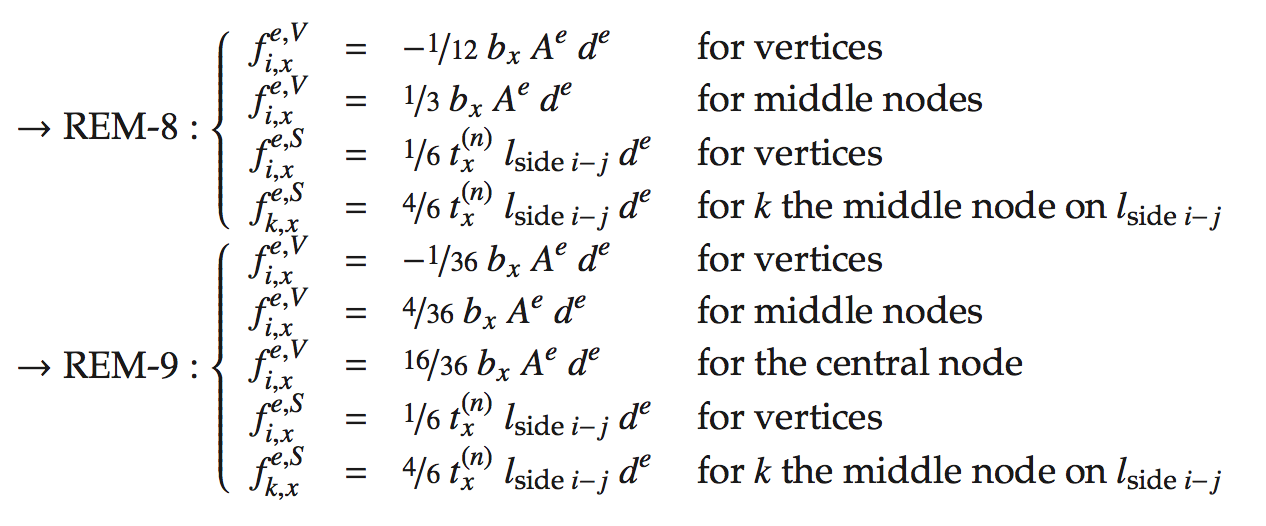
\includegraphics[scale=0.4]{ch2/11}
					\captionof{figure}{}
					\end{wrapfigure}
					The force at the pressure center P is equivalent to another force in point Q, but by adding the momentum to compensate the one added by moving the force. This momentum is:
					
					\begin{equation}
					\vec{C_Q} = -\vec{PQ}\times \vec{R}.
					\end{equation}
					
				\subsubsection{Aerodynamic center}
					Suppose that there is a point Q where this couple $C_Q$ is independent of the angle of attack (because the pressure center changes with alpha). This point is called the aerodynamic center. We have to show that this exists. For this way:
					\begin{enumerate}
						\item We will begin by calculating the center of pressure by integrating the pressure field. We can calculate the magnitude, but not the acting point. 
						
						\item We compute the momentum of the pressure forces around the leading edge (\autoref{fig:2.11}):
						
						\begin{equation}
						\vec{M}_{LE} = \oint \vec{OQ} \times d\vec{F} = \underbrace{M_{LE}}_{<0} \vec{1}_z 
						\end{equation}
						where $\vec{1}_z$ goes in the paper. 						
						
						\item On the other hand, we know that $\vec{R}$ has a certain direction with a normal component, so we can make the momentum (\autoref{fig:2.12}): 
						
						\begin{equation}
						M_{LE} = -x_p.N
						\end{equation}
					\end{enumerate}
					
					By using point 2 and 3 we can find $x_{p}$.
					
					\begin{center}
					\begin{minipage}{0.4\textwidth}
					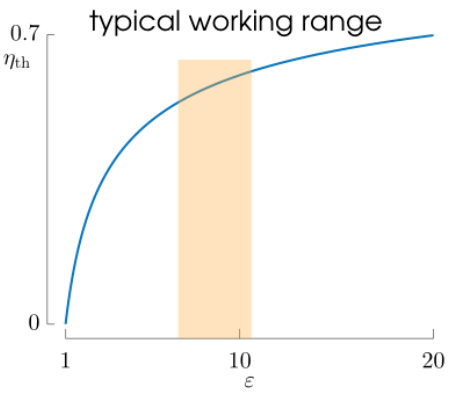
\includegraphics[scale=0.65]{ch2/12}
					\captionof{figure}{}
					\label{fig:2.11}
					\end{minipage}
					\begin{minipage}{0.4\textwidth}
					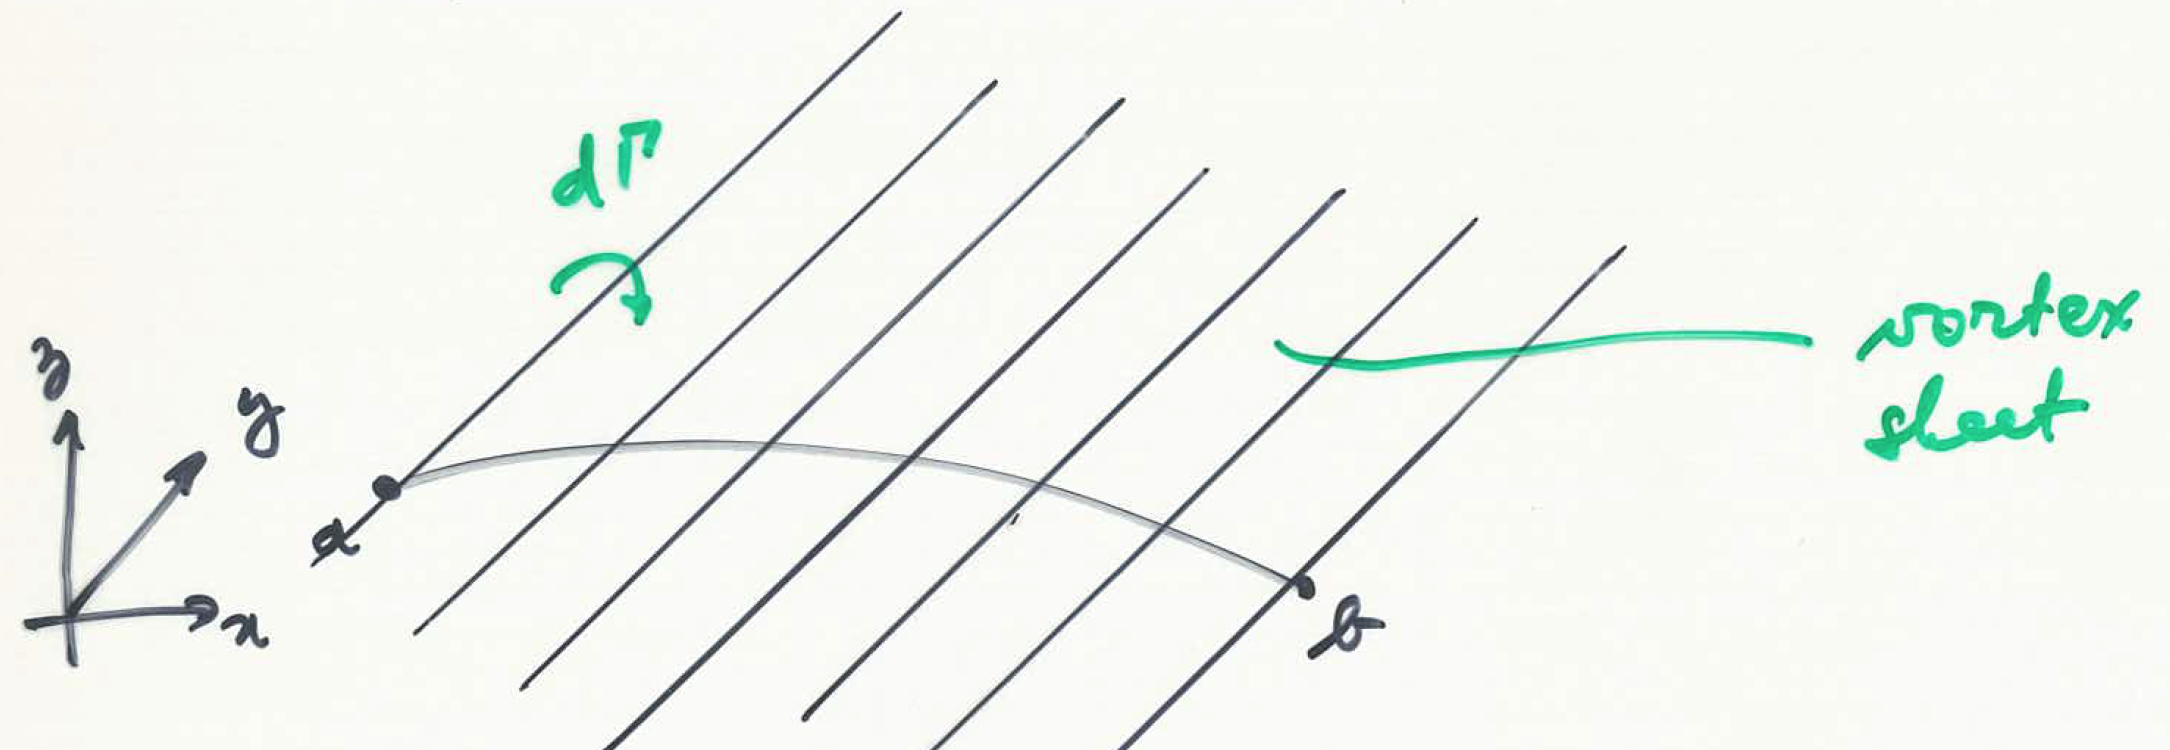
\includegraphics[scale=0.6]{ch2/13}
					\captionof{figure}{}
					\label{fig:2.12}
					\end{minipage}
					\end{center}